\documentclass[main.tex]{subfiles}
\begin{document}

\section{Sheet 2}

\subsection{Constant acceleration}

\subsubsection{Coordinate velocity}

We are given the position as a function of time, 
\begin{equation} \label{eq:constant-acceleration} 
  x(t) = \frac{\sqrt{1 + \kappa^2 t^2} -1 }{\kappa }\,,
\end{equation}
%
and we can directly compute its derivative
%
\begin{equation} \label{eq:constant-acceleration-velocity} 
  v(t) = \dv{x}{t} =
  \frac{\kappa t}{\sqrt{\kappa^2 t^2  + 1} }\,.
\end{equation}

It is clear from the expression that \(\abs{v} < 1\) for all times, while \(v\) approaches 1 at positive temporal infinity and \(-1\) at negative temporal infinity.

\begin{figure}[h]
    \centering
    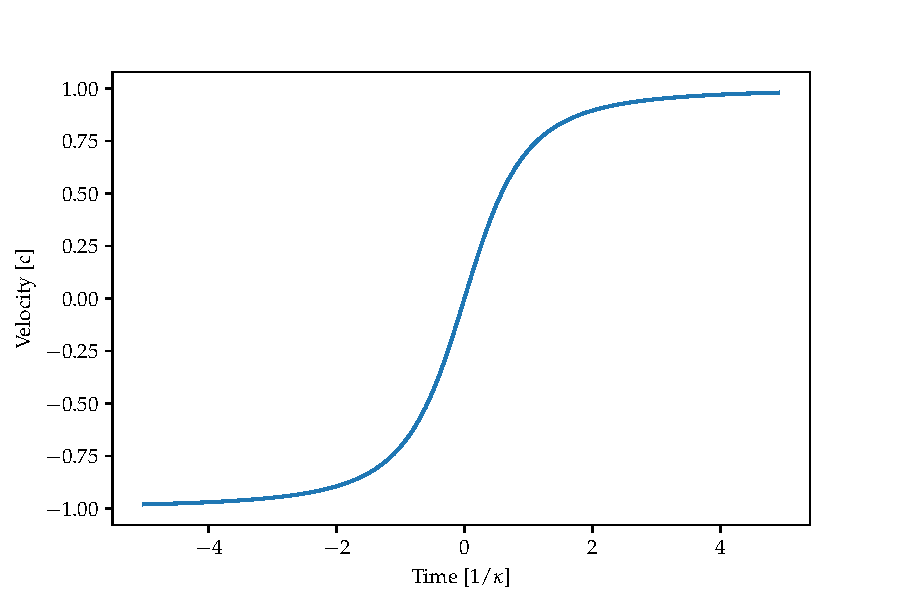
\includegraphics[width=\textwidth]{figures/velocity.pdf}
    \caption{Velocity as a function of coordinate time \(t\)}
    \label{fig:velocity-constant-acceleration}
\end{figure}

\subsubsection{Components of the 4-velocity}

The Lorentz factor \(\gamma \) is given by
%
\begin{equation} \label{eq:constant-acceleration-gamma}
  \gamma = \frac{1}{\sqrt{1-v^2}}
  = \frac{1}{\sqrt{1 - \frac{\kappa^{2} t^{2}}{\kappa^{2} t^{2} + 1} }}
  = \sqrt{\kappa^2 t^2 + 1} \,,
\end{equation}
%
therefore the four-velocity is given by:
%
\begin{equation}
  u^{\mu } =
  \begin{bmatrix}
  \gamma  \\
  \gamma v \\
  0 \\
  0
  \end{bmatrix}
  =
  \begin{bmatrix}
    \sqrt{\kappa^2 t^2 + 1}  \\
    \kappa t \\
    0 \\
    0
  \end{bmatrix}\,.
\end{equation}

\subsubsection{Proper time}

The relation between coordinate and proper time is given by the definition of the first component of the four-velocity: \(u^{0} = \dv*{t}{\tau} = \gamma \), therefore \(\dd{\tau } = \dd{t} / \gamma \).
Integrating this relation we get:
%
\begin{equation}
    \tau = \int \dd{\tau } 
    = \int \frac{\dd[]{t} }{\gamma }
    = \displaystyle \frac{\operatorname{arcsinh}{\left(\kappa t \right)}}{\kappa}\,,
\end{equation}
%
where the constant of integration is selected by imposing \(t = 0 \iff \tau = 0\).
Notice that, as we would expect, when expanding up to second order near \(t = \tau = 0 \) we have \(t \sim \tau \), since in that region the velocity is much less than unity.

The inverse relation is given by \(t = \sinh (\kappa \tau ) / \kappa \). Using this, we can write:
%
\begin{equation}
  x (t(\tau ))  =\frac{\cosh{\left(\kappa \tau \right)} - 1}{\kappa}\,.
\end{equation}

\subsubsection{Four-acceleration}

Now, we wish to compute the four-acceleration. There are many ways to approach this: an easy one is to simply find the explicit expression \(u^{\mu } (\tau )\) and to differentiate it. The expression we get is:
%
\begin{equation}
    a^{\mu } = \dv{}{\tau } u^{\mu } = \dv{}{\tau }   
  \begin{bmatrix}
    \sqrt{\sinh^{2}{\left(\kappa \tau \right)} + 1}
        \\
    \frac{\sqrt{\kappa^{2} t^{2} + 1} \sinh{\left(\kappa \tau \right)}}{\sqrt{\sinh^{2}{\left(\kappa \tau \right)} + 1}} \\
    0 \\
    0
  \end{bmatrix}
  =
  \begin{bmatrix}
    \frac{\sqrt{2} \kappa \sinh{\left(2 \kappa \tau \right)}}{2 \sqrt{\cosh{\left(2 \kappa \tau \right)} + 1}}
    \\
    \kappa \cosh \left(\kappa \tau \right)\\
    0 \\
    0
  \end{bmatrix}
\,,
\end{equation}
%
which is a bit unwieldy but it can be used to check two important facts: \(a^{\mu } a_{\mu } = \const \) and \(a^{\mu }u_{\mu } = 0\). The first of the two is:
%
\begin{equation}
    a^{\mu }a_{\mu } = -(a_0 )^2 + (a_1 )^2 =
    \kappa^{2} \cosh^{2}{\left(\kappa \tau \right)} - \frac{\kappa^{2} \sinh^{2}{\left(2 \kappa \tau \right)}}{2 \left(\cosh{\left(2 \kappa \tau \right)} + 1\right)}
    = \kappa^2 
\,,
\end{equation}
%
which tells us that the constant acceleration \(\sqrt{a^{\mu }a_{\mu }} = \kappa \).

Also, we verify the orthogonality to the four-velocity: 
%
\begin{equation}
  a^{\mu }u_{\mu } = 
  - \frac{\sqrt{2} \kappa \sqrt{\sinh^{2}{\left(\kappa \tau \right)} + 1} \sinh{\left(2 \kappa \tau \right)}}{2 \sqrt{\cosh{\left(2 \kappa \tau \right)} + 1}} + \kappa \sinh{\left(\kappa \tau \right)} \cosh{\left(\kappa \tau \right)}
  = 0
\,.
\end{equation}

\subsubsection{Local velocity \& acceleration}

We can apply a Lorentz boost corresponding to this velocity:
it will be given by the matrix:
%
\begin{equation}
  \left[\begin{array}{cccc}
  \gamma  & -v \gamma  & 0 & 0 \\ 
  -v \gamma  & \gamma  & 0 & 0 \\ 
  0 & 0 & 1 & 0 \\ 
  0 & 0 & 0 & 1
  \end{array}\right]
\,,
\end{equation}
%
where \(v\) and \(\gamma \) are those found before.
Without doing any calculations we could already say that the transformed velocity will be equal to the time-like unit vector, while the acceleration will be equal to \(\kappa \) times the unit \(x\)-directed vector.

The velocity becomes:
%
\begin{equation}
  \qty(u^{\mu})' =
  \left[\begin{array}{cccc}
    \sqrt{\kappa^2 t^2 + 1}  & -\kappa t  & 0 & 0 \\ 
    -\kappa t  & \sqrt{\kappa^2 t^2 + 1}  & 0 & 0 \\ 
    0 & 0 & 1 & 0 \\ 
    0 & 0 & 0 & 1
    \end{array}\right]
    \begin{bmatrix}
      \sqrt{\kappa^2 t^2 + 1}  \\
      \kappa t \\
      0 \\
      0
    \end{bmatrix} 
  = 
  \begin{bmatrix}
  1 \\
  0 \\
  0 \\
  0
  \end{bmatrix}
\,,
\end{equation}
%
as we expected.

The acceleration instead becomes:
%
\begin{equation}
  \qty(a^{\mu})' =
  \left[\begin{array}{cccc}
    \sqrt{\kappa^2 t^2 + 1}  & -\kappa t  & 0 & 0 \\ 
    -\kappa t  & \sqrt{\kappa^2 t^2 + 1}  & 0 & 0 \\ 
    0 & 0 & 1 & 0 \\ 
    0 & 0 & 0 & 1
    \end{array}\right]
    \begin{bmatrix}
      \frac{\sqrt{2} \kappa \sinh{\left(2 \kappa \tau \right)}}{2 \sqrt{\cosh{\left(2 \kappa \tau \right)} + 1}}
      \\
      \kappa \cosh \left(\kappa \tau \right)\\
      0 \\
      0
    \end{bmatrix}
  = 
  \begin{bmatrix}
  0 \\
  \kappa  \\
  0 \\
  0
  \end{bmatrix}
\,,
\end{equation}
%

\subsection{Fixed target collision}

\subsubsection{Center of mass momenta}

In the CoM frame, the momenta of the two protons are respectively \((E_p, \pm p, 0,0)^\top = m_p (\gamma, \pm v, 0, 0)\), where \(E_p^2 = m_p^2 + p^2\).
The total CoM energy is \(-(p^\mu _A + p^\mu _B )^2 = 2 m_p^2\).

\subsubsection{Center of mass velocity}

The momentum of particle \(B\) will be given by \(p^{\mu } = m_p u^{\mu } = (m_p \gamma , m_p \gamma v, 0, 0)^\top\). Therefore, \(\gamma v = p / m_p\). Solving this we get: 
%
\begin{equation}
  v = \frac{p}{m_p} \sqrt{\frac{1}{(p/m_p)^{2} + 1}} = \frac{p}{E_p}
\,,
\end{equation}
%

\subsubsection{Lab frame momenta}

The momentum of particle \(B\) in its own rest frame will just be \((m_p, 0, 0, 0)^\top\).
The momentum of particle \(A\) instead will be given by a boost in the \(x\) direction with velocity \(-v\):
%
\begin{equation}
  (p_A^\mu) _{\text{lab}} = 
  \left[\begin{array}{cccc}
  \gamma  & v \gamma  & 0 & 0 \\ 
  v \gamma  & \gamma  & 0 & 0 \\ 
  0 & 0 & 1 & 0 \\ 
  0 & 0 & 0 & 1
  \end{array}\right]
  \left[\begin{array}{c}
  E_p  \\ 
  p \\ 
  0 \\ 
  0
  \end{array}\right]  
  = \left[\begin{array}{c}
    \gamma E_p + v \gamma p  \\ 
    v \gamma E_p + \gamma p \\ 
    0 \\ 
    0
    \end{array}\right]  
  = \left[\begin{array}{c}
    m_p \frac{1+v^2}{\sqrt{1-v^2}}  \\ 
    2 \gamma p\\ 
    0 \\ 
    0
    \end{array}\right]
\,,
\end{equation}
%

\subsection{Weak field gravitational time dilation}

\subsubsection{Time dilation expression}

It is more intuitive geometrically to deal with a pulse sent from \(A\) to \(B\), for which we expect the time dilation to work in the opposite sense: 
%
\begin{equation}
  \Delta t_B = \Delta t_A \qty(1 + gh)
\,,
\end{equation}
%
up to first order in \(gh\) and \(g\Delta t_A\), since \((1+gh )(1-gh) = 1-(gh)^2 = 1\) to first order in \(gh\).

We know that the paths of the observers are two curves of constant acceleration: we know their explicit expression from equation \eqref{eq:constant-acceleration}, and additionally we assume that they are separated by a space interval \(h\): 
%
\begin{subequations}
\begin{align}
  x_A(t) &= \frac{\sqrt{1 + (gt)^2} -1}{g} \\ 
  x_B(t) &= \frac{\sqrt{1 + (gt)^2} -1}{g} + h
  \,.
\end{align}
\end{subequations}

At \(t=0\) Alice sends a pulse, which then reaches Bob at a time \(t_1\). After a time \(\Delta t_A\), she sends another, which then reaches Bob at a time \(t_2 \). 
Right now, we are referring to all times as measured in the rest frame of Alice at \(t=0\).
These times can be found by imposing that the space and time separation between the events of the pulse being sent and received are equal, since it travels at light speed: the equations which represent this are \(x_B(t_1) = t_1\) and \(x_B(t_2 ) -x_A (\Delta t_A) = t_2 - \Delta t_A\). Substituting the expressions for the positions:
%
\begin{subequations}
\begin{align}
  t_1 &= \frac{\sqrt{1+(g t_1 )^2} -1}{g} +h \\
  t_2 - \Delta t_A &= \frac{\sqrt{1+(gt_2 )^2} -1}{g} + h - \qty(\frac{\sqrt{1+(g \Delta t_A )^2} -1}{g})\,.
\end{align}
\end{subequations}

Now, it is just a matter of calculation to solve these equations, expand up to first order in the adimensional parameters \(gh\) and \(g \Delta t_A\) and one recovers the desidered expression for  \(\Delta t_B = t_2 - t_1\).

There is one more consideration to make though: what about the Lorentz time dilation for Bob? This it actually a \emph{second order effect}.

\begin{claim}
The time interval measured by Bob in his frame at \(t \sim t_1\) is the same as the one measured in the rest frame of Alice at \(t=0\) up to first order in \(gh\) and \(g \Delta t_B\).
\end{claim}

\begin{proof}
We perform a Lorentz boost to the velocity of Bob at \(t=t_1 \): this is given by equation \eqref{eq:constant-acceleration-velocity}, and is equal to:
%
\begin{equation}
  v = \frac{gt }{\sqrt{(gt)^2 + 1}}
\,,
\end{equation}
%
with a Lorentz factor of \(\gamma = \sqrt{(gt)^2 +1} \) (see equation \eqref{eq:constant-acceleration-gamma}).

The temporal separation between the two events is \(\Delta t_B\), while the spatial separation is \(\Delta x_B \approx  v \Delta t_B\) to first order. The boost, in the \((t, x)\) plane, looks like: 
%
\begin{equation}
  \left[\begin{array}{c}
  \Delta t_B \\ 
  \Delta x_B
  \end{array}\right]'
  =
  \left[\begin{array}{cc}
  \gamma  & -v \gamma  \\ 
  -v \gamma  & \gamma 
  \end{array}\right]  
  \left[\begin{array}{c}
  \Delta t_B \\ 
  \Delta x_B
  \end{array}\right] 
  =
  \left[\begin{array}{c}
  \Delta t_B \qty(\sqrt{(gt)^2+1} - (gt)^2/\sqrt{(gt)^2+1}) \\ 
  -gt \Delta t_B + \sqrt{(gt)^2+1} gt \Delta t / \sqrt{(gt)^2+1}
  \end{array}\right]
\,,
\end{equation}
%
therefore as we would expect the spatial separation is eliminated, while expanding the factor multiplying the temporal one near \(gt = 0\) we get: 
%
\begin{equation}
  \sqrt{(gt)^2+1} - (gt)^2/\sqrt{(gt)^2+1} = 1+O((gt)^2)
\,,
\end{equation}
%
which proves our result.
\end{proof}

\subsubsection{Gravitational time dilation}

By the equivalence principle, the effects measured in a uniformly accelerating frame at \(g\) are the same as those measured in a gravitational field with constant acceleration \(g\).
The gravitational field in such a frame is given by \(\Phi  = gh\), where \(h\) is the height (with arbitrary zero point): the result follows.

\subsubsection{Twins and gravitation}

The gravitational time dilation difference, in absolute value, is given by: 
%
\begin{equation}
  \Delta t = t _{\text{elapsed}} \frac{g \Delta h}{c^2}
  \approx \SI{1}{yr} \frac{\SI{10}{m/s} \times \SI{100}{m}}{(\SI{3e8}{m/s})^2} \approx \SI{3.5e-7}{s} 
\,.
\end{equation}

We are asked what is the age of the twin on the ground as measured by the twin who is higher up: this is analogous to the situation considered in the first section of this problem; the twin higher up will measure the twin lower down to be 
%
\begin{equation}
  \SI{1}{yr} + \SI{3.5e-7}{s} \approx (1+\num{1e-14}) \SI{}{yr} 
\,
\end{equation}
%
old.

\end{document}